\documentclass[12pt]{article}

\usepackage{setspace}
\usepackage{caption}
\usepackage{subcaption}
\usepackage{float}
\usepackage{makecell}
\usepackage{amsmath}
\usepackage{graphicx}
\usepackage{subfig}
\graphicspath{ {./images/} }
\usepackage[utf8]{inputenc}
\usepackage[russian]{babel}
\usepackage{geometry}
 \geometry{
 a4paper,
 left=20mm,
 right=20mm,
 top=20mm,
 bot=20mm,
 }

\begin{document}

\begin{titlepage}
\begin{center}
    НАЦИОНАЛЬНЫЙ ИССЛЕДОВАТЕЛЬСКИЙ УНИВЕРСИТЕТ ИТМО \\
    Факультет систем управления и робототехники \\
    \vspace*{10\baselineskip}
    {\LARGEЭлектротехника} \\
    \ \\
    \ \\
    \begin{spacing}{1.5}
    {\large Лабораторная работа №3 \\
    ИССЛЕДОВАНИЕ НЕЛИНЕЙНЫХ ЦЕПЕЙ \\
    \ \\
    Вариант 3R382}
    \end{spacing} \\
    \ \\
    \vspace*{10\baselineskip}
    \hfill {Студент: Кирбаба Д.Д.\ \ \ \ \ \ \ \ \ } \\
    \hfill {Группа: R3338\ \ \ \ \ \ \ \ \ \ \ \ \ \ \ \ \ \ \ \ \ } \\
    \hfill {Преподаватель: Китаев Ю.В.} \\
    \mbox{}
    \vfill {г. Санкт-Петербург\\2023}
\end{center}
\end{titlepage}

\subsubsection*{Цель работы}
Снятие прямых и обратных вольт-амперных характеристик(ВАХ) диодов.

\subsubsection*{Ход работы}
\begin{figure}[H]
    \centering
    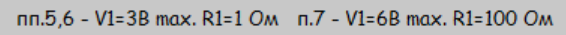
\includegraphics[width=0.5\textwidth]{initials.png}
    \caption{Начальные данные.}
    \label{fig:initials}
\end{figure}

Исследуем вольт-амперные характеристики прямого прохода диодов SB320 и 1N4001GP, используя данную схему:
\begin{figure}[H]
    \centering
    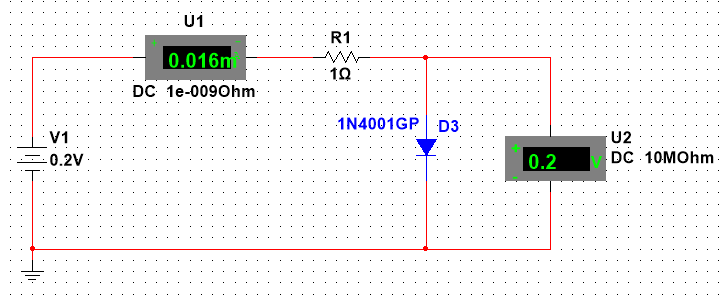
\includegraphics[width=0.7\textwidth]{dir_scheme_1_2.png}
    \caption{Схема моделирования прямого прохода.}
    \label{fig:dir_scheme_1_2}
\end{figure}

Последовательно задавая напряжение на источнике V1 от $0.2 \ V$ до $3 \ V$ с шагом $0.2 \ V$ будем производить измерения напряжения и силы тока на диоде:
\begin{figure}[H]
    \centering
    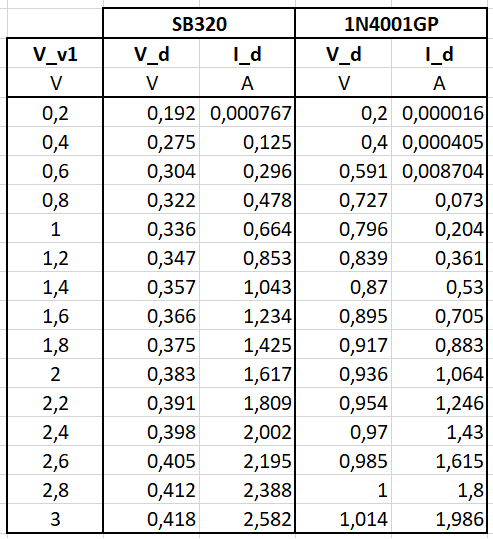
\includegraphics[width=0.5\textwidth]{table_dir_1_2.png}
    \caption{Таблица измерений при прямом проходе.}
    \label{fig:table_dir_1_2}
\end{figure}

По данным значениям построим график зависимости тока $I_d$ от напряжения $V_d$ на диоде при различных значениях входного напряжения $V_v1$:
\begin{figure}[H]
    \centering
    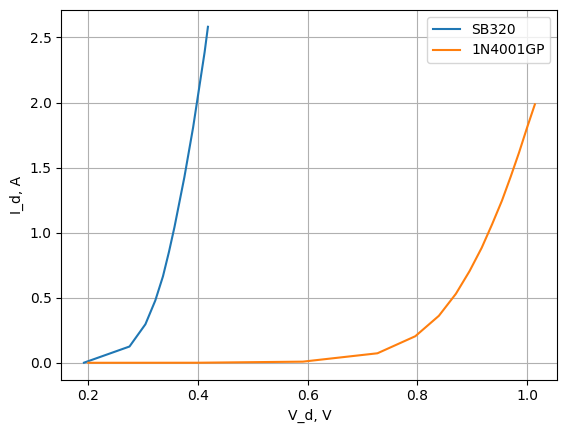
\includegraphics[width=0.8\textwidth]{vac_1_2_dir.png}
    \caption{ВАХ прямого прохода диодов SB320 и 1N4001GP.}
    \label{fig:vac_1_2_dir}
\end{figure}

Таким же образом исследуем поведение ВАХ при прямом проходе следующих диодов: $LED_{red}$ и $LED_{blue}$. Для этого установим сопротивление $100 \ Ohm$:
\begin{figure}[H]
    \centering
    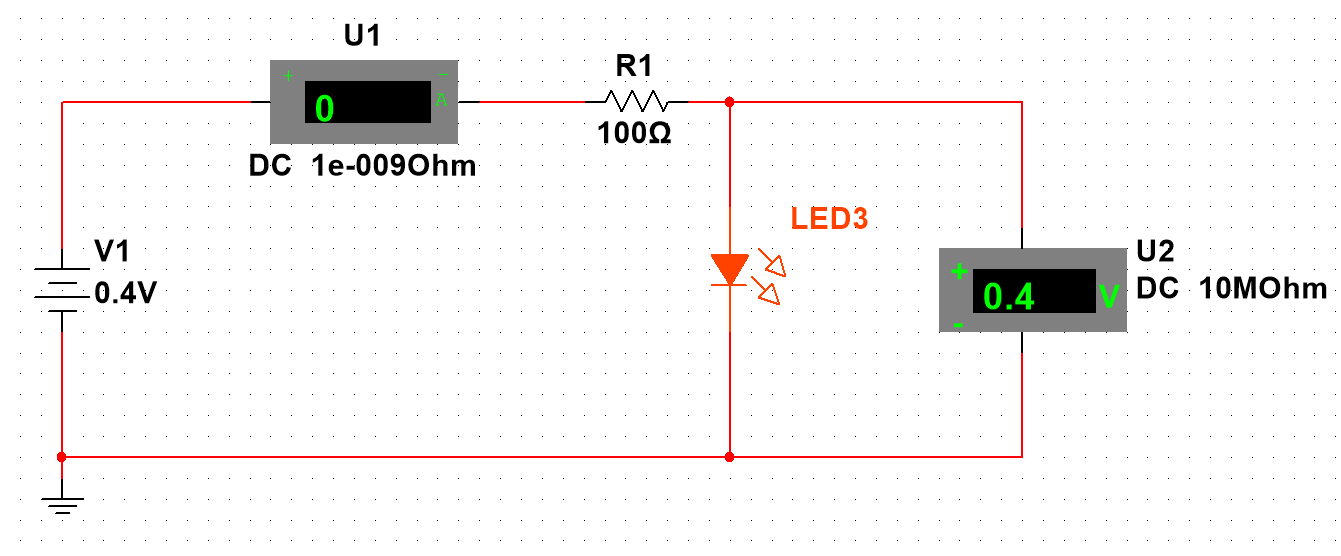
\includegraphics[width=0.7\textwidth]{dir_scheme_b_r.png}
    \caption{Схема моделирования прямого прохода.}
    \label{fig:dir_scheme_b_r}
\end{figure}

Последовательно задавая напряжение на источнике V1 от $0.4 \ V$ до $6 \ V$ с шагом $0.4 \ V$ будем производить измерения напряжения и силы тока на диоде:
\begin{figure}[H]
    \centering
    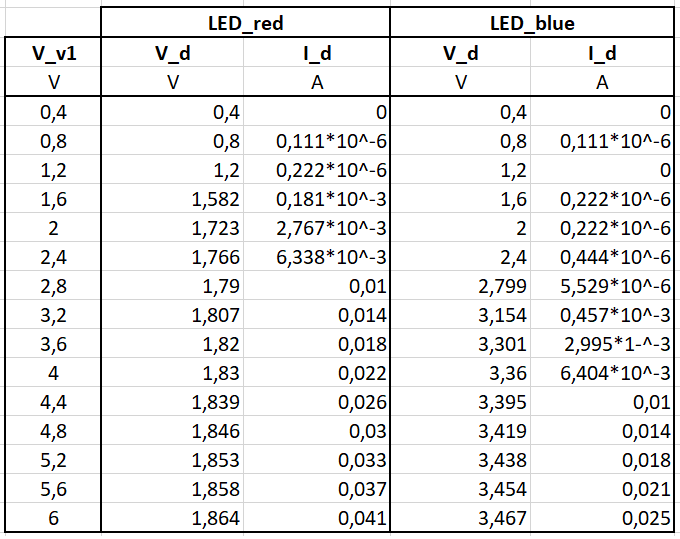
\includegraphics[width=0.5\textwidth]{table_dir_b_r.png}
    \caption{Таблица измерений при прямом проходе.}
    \label{fig:table_dir_b_r} 
\end{figure}

По данным значениям построим график зависимости тока $I_d$ от напряжения $V_d$ на диоде при различных значениях входного напряжения $V_v1$:
\begin{figure}[H]
    \centering
    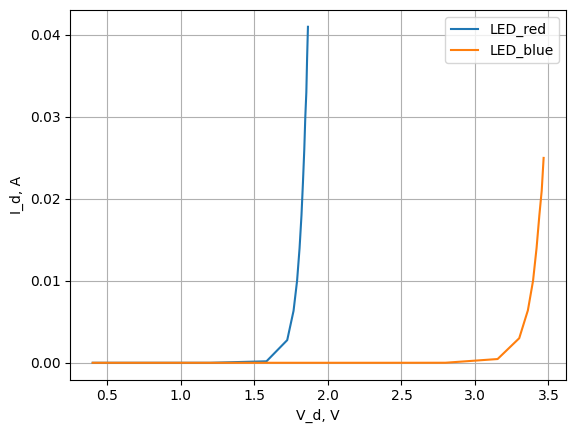
\includegraphics[width=0.8\textwidth]{vac_b_r_dir.png}
    \caption{ВАХ прямого прохода диодов $LED_{red}$ и $LED_{blue}$.}
    \label{fig:vac_b_r_dir}
\end{figure}

Диапазоны предельно допустимых значений:
\begin{center}
\begin{tabular}{ c|c c c c } 
   & SB320 & 1N4001GP & $LED_{red}$ & $LED_{blue}$ \\ 
   \hline
  $I_{d_{max}}, \ A$ & $3$ & $1$ & $0.03$ & $0.03$ \\ 
  $V_{d_{max}}, \ V$ & $200$ & $1.1$ & $2.2$ & $4$ \\ 
\end{tabular}
\end{center}

Отметим выпадающие из диапазона точки на ВАХ:
\begin{figure}[H]
    \centering
        \subfloat[\centering SB320, 1N4001GP]{{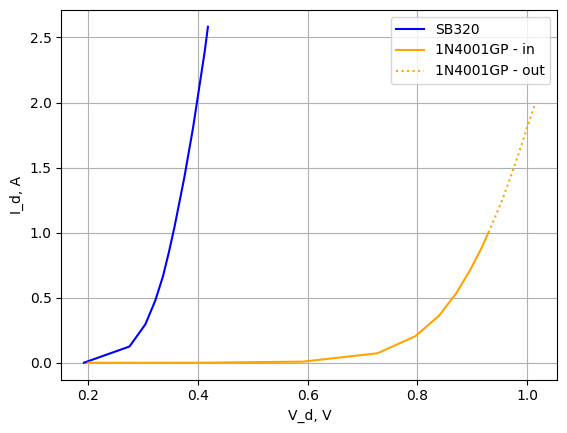
\includegraphics[width=0.45\textwidth]{vac_1_2_dir_color.png} }}%
        \qquad
        \subfloat[\centering $LED_{red}$, $LED_{blue}$]{{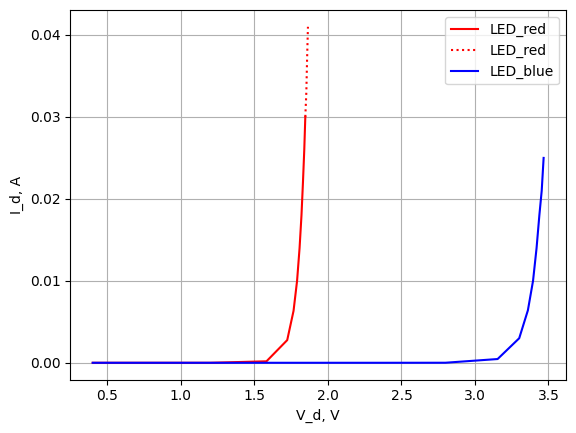
\includegraphics[width=0.45\textwidth]{vac_b_r_dir_color.png} }}%
        \caption{Прямые ВАХ с диапазоном.}%
    \label{fig:example}
\end{figure}

Теперь проведем такие же манипуляции для исследования обратных ВАХ данных диодов. \\
Необходимо только подавать напряжение в обратной полярности и убрать резистор:
\begin{figure}[H]
    \centering
    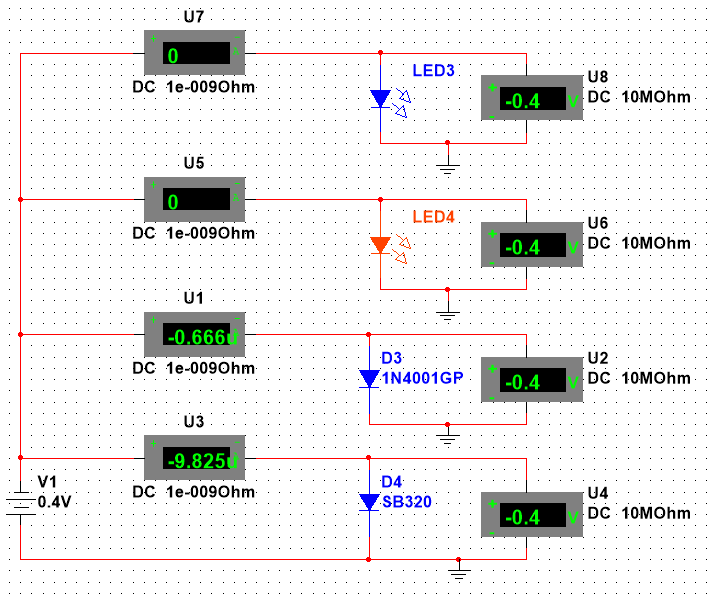
\includegraphics[width=0.7\textwidth]{inv_scheme_all.png}
    \caption{Схема моделирования обратного прохода диодов.}
    \label{fig:inv_scheme_all}
\end{figure}

Последовательно задавая напряжение на источнике V1 от $0.4 \ V$ до $6 \ V$ с шагом $0.4 \ V$ будем производить измерения напряжения и силы тока на диодах:
\begin{figure}[H]
    \centering
    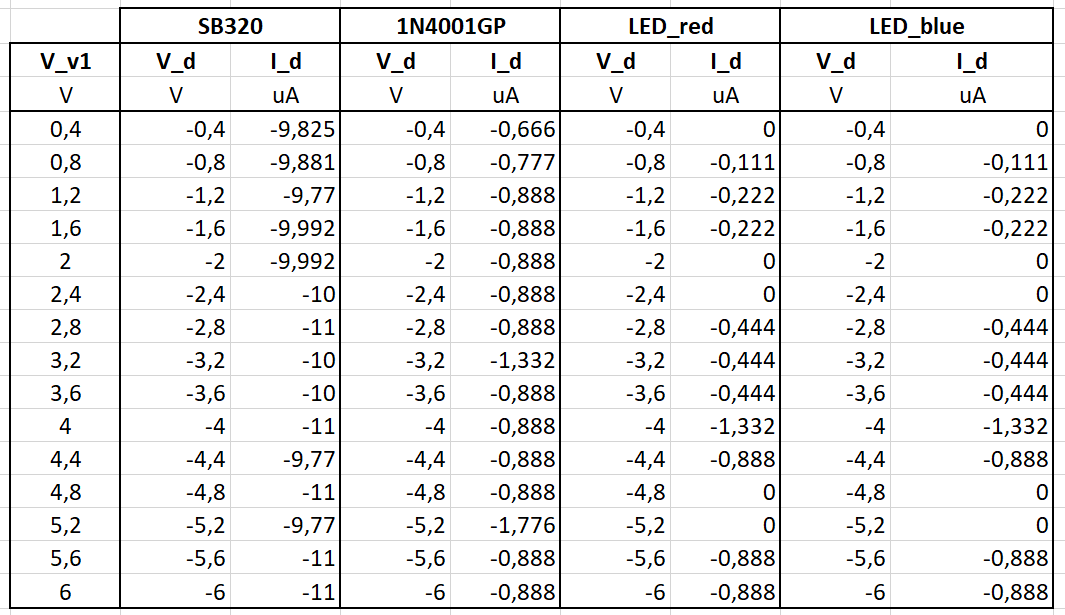
\includegraphics[width=0.5\textwidth]{table_inv_all.png}
    \caption{Таблица измерений при обратном проходе.}
    \label{fig:table_inv_all} 
\end{figure}

По данным значениям построим график зависимости тока $I_d$ от напряжения $V_d$ на диодах при различных значениях входного напряжения $V_v1$:
\begin{figure}[H]
    \centering
    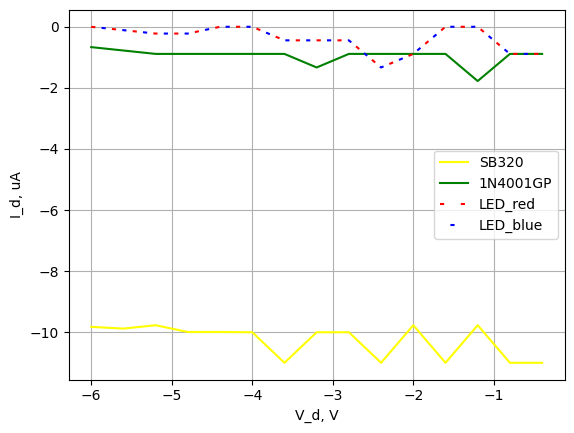
\includegraphics[width=0.8\textwidth]{vac_inv_all.png}
    \caption{ВАХ обратного прохода диодов.}
    \label{fig:vac_inv_all}
\end{figure}

Получим ВАХ с помощью осциллографа:
\begin{figure}[H]
    \centering
    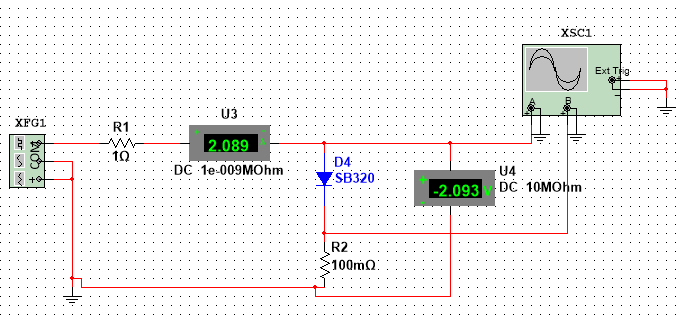
\includegraphics[width=0.7\textwidth]{osc_cheme.png}
    \caption{Схема моделирования ВАХ с помощью осциллографа.}
    \label{fig:osc_cheme}
\end{figure}

\begin{figure}[H]
    \centering
        \subfloat[\centering SB320]{{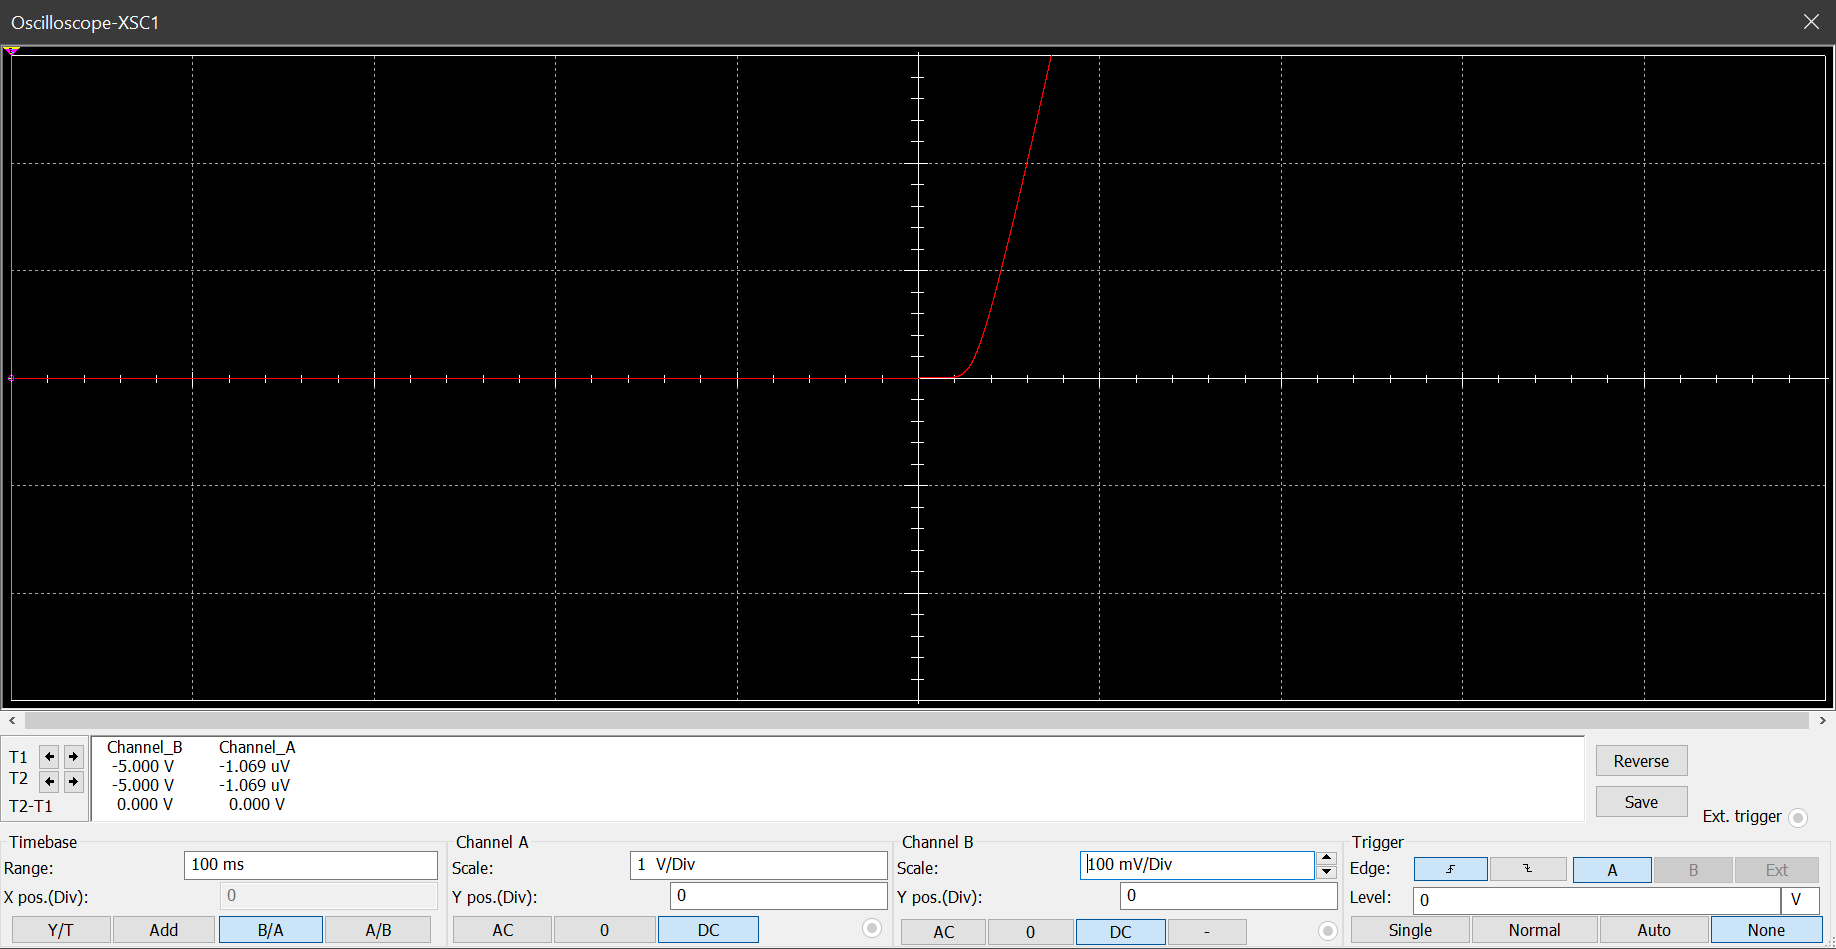
\includegraphics[width=0.45\textwidth]{sb_osc.png} }}%
        \qquad
        \subfloat[\centering 1N4001GP]{{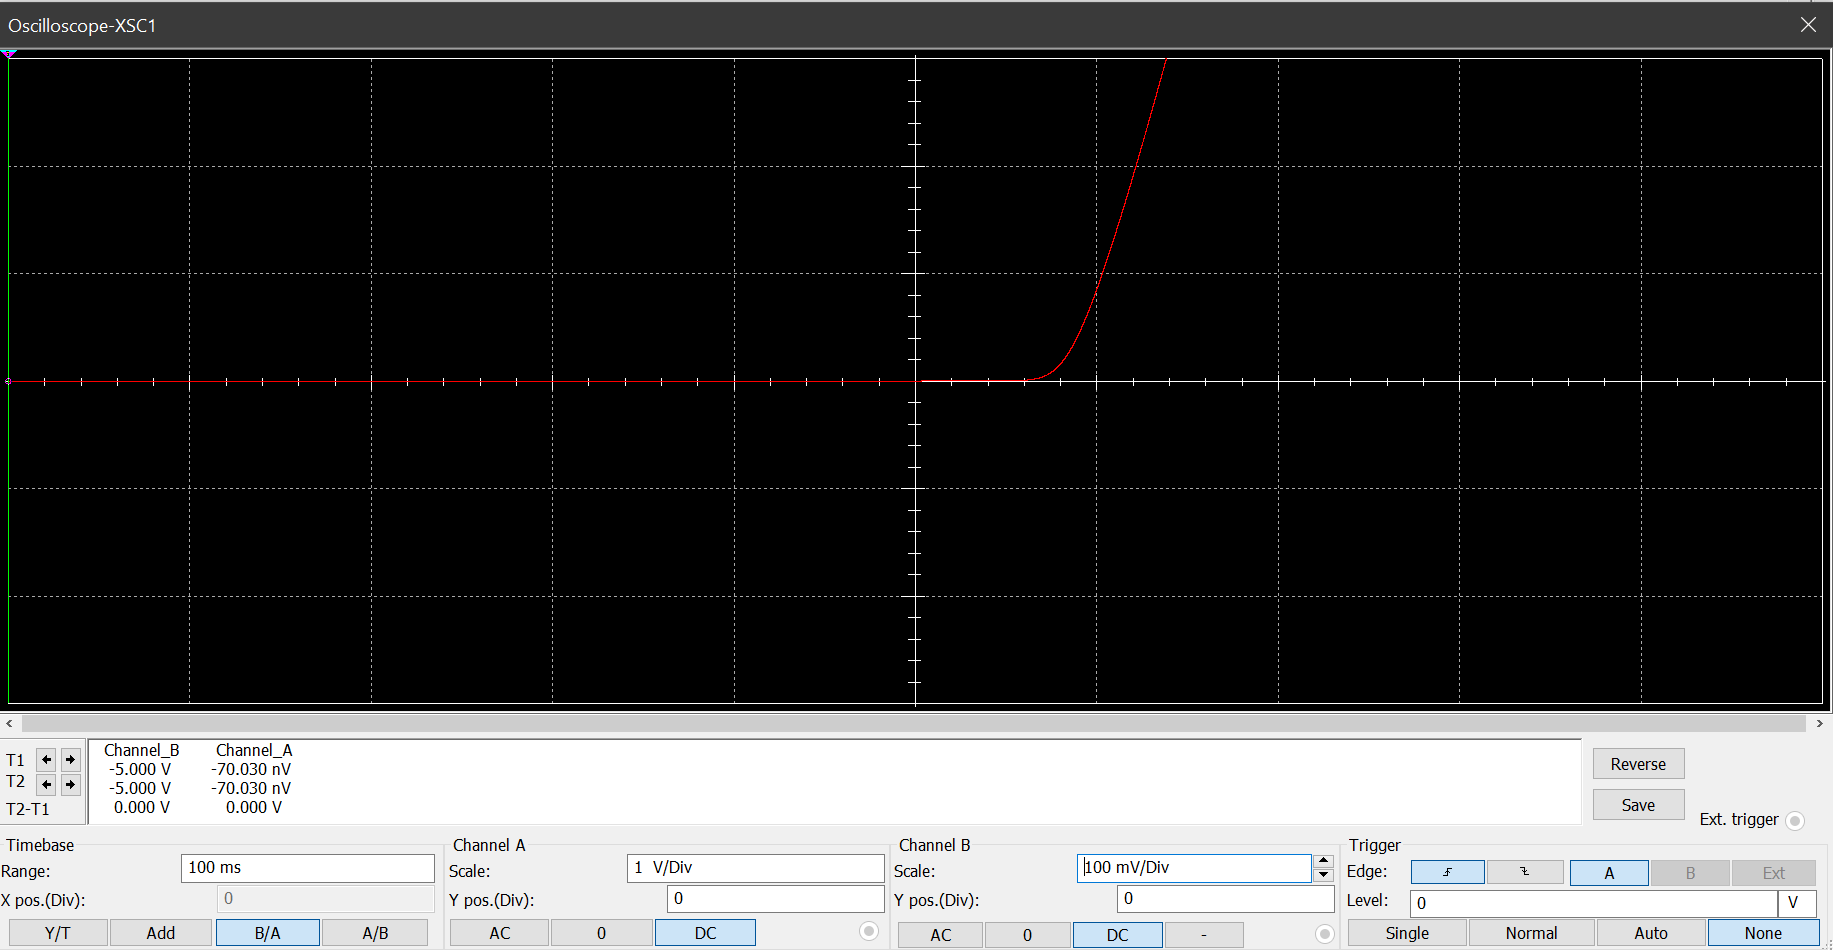
\includegraphics[width=0.45\textwidth]{1n_osc.png} }}%
        \caption{ВАХ с осциллограммы.}%
    \label{fig:example}
\end{figure}

\begin{figure}[H]
    \centering
        \subfloat[\centering $LED_{red}$]{{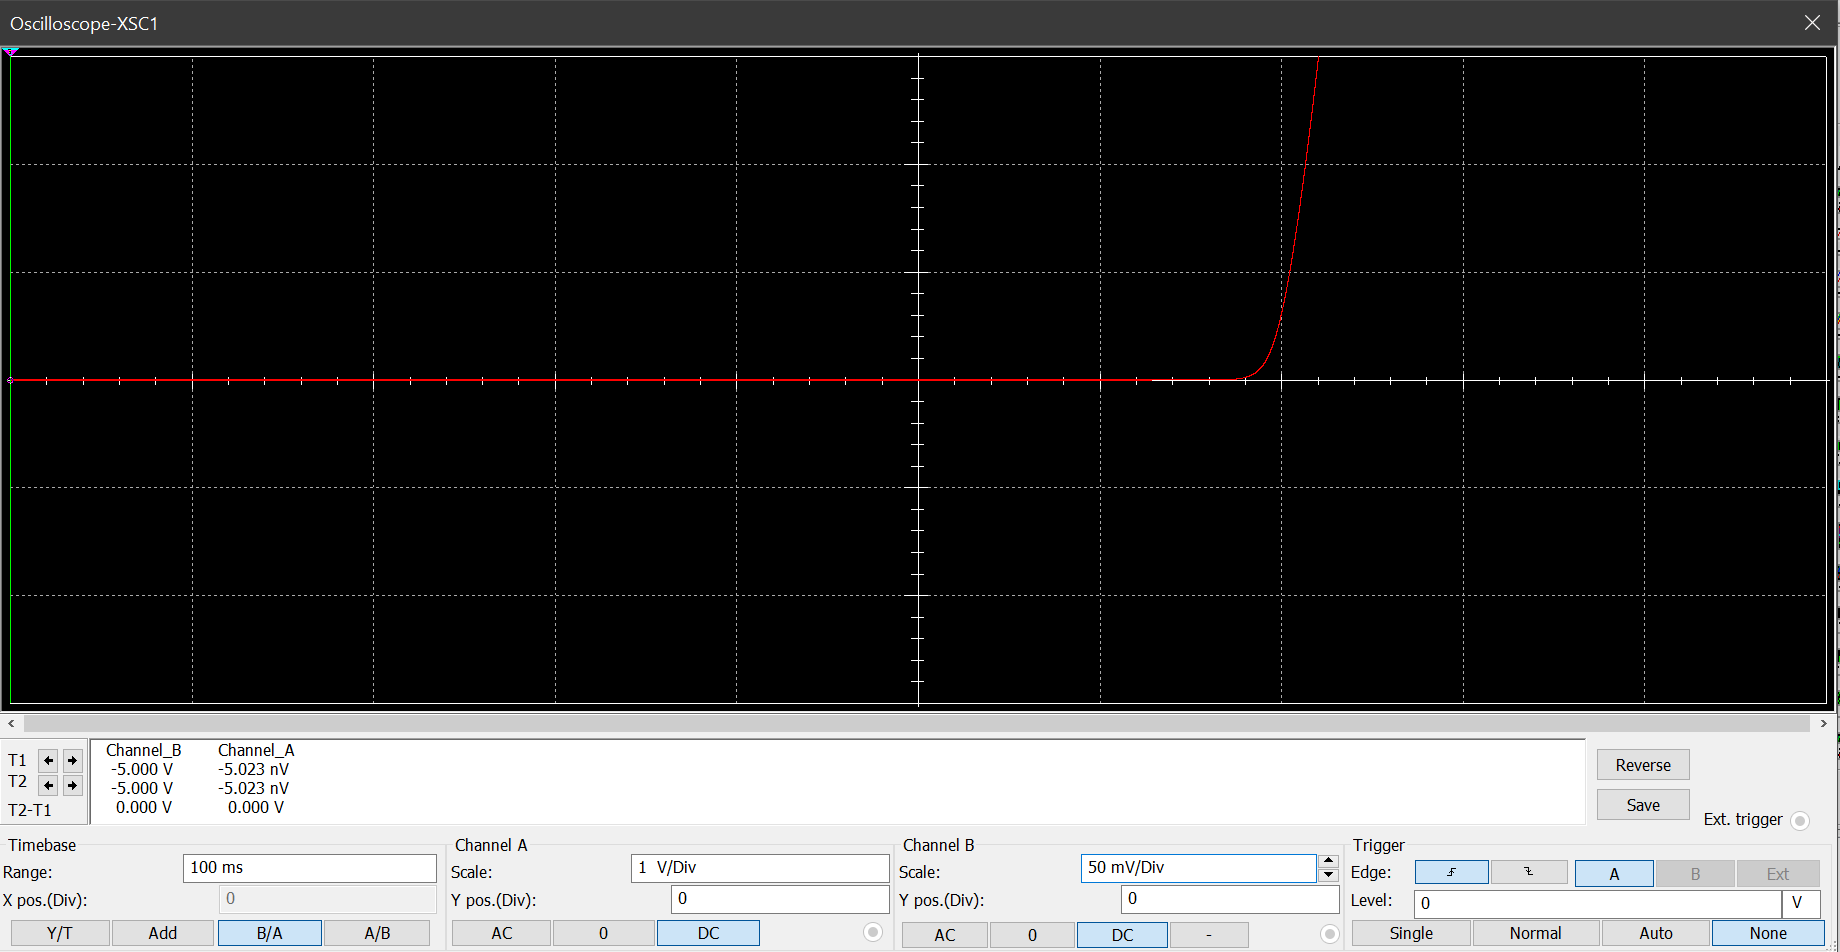
\includegraphics[width=0.45\textwidth]{red_osc.png} }}%
        \qquad
        \subfloat[\centering $LED_{blue}$]{{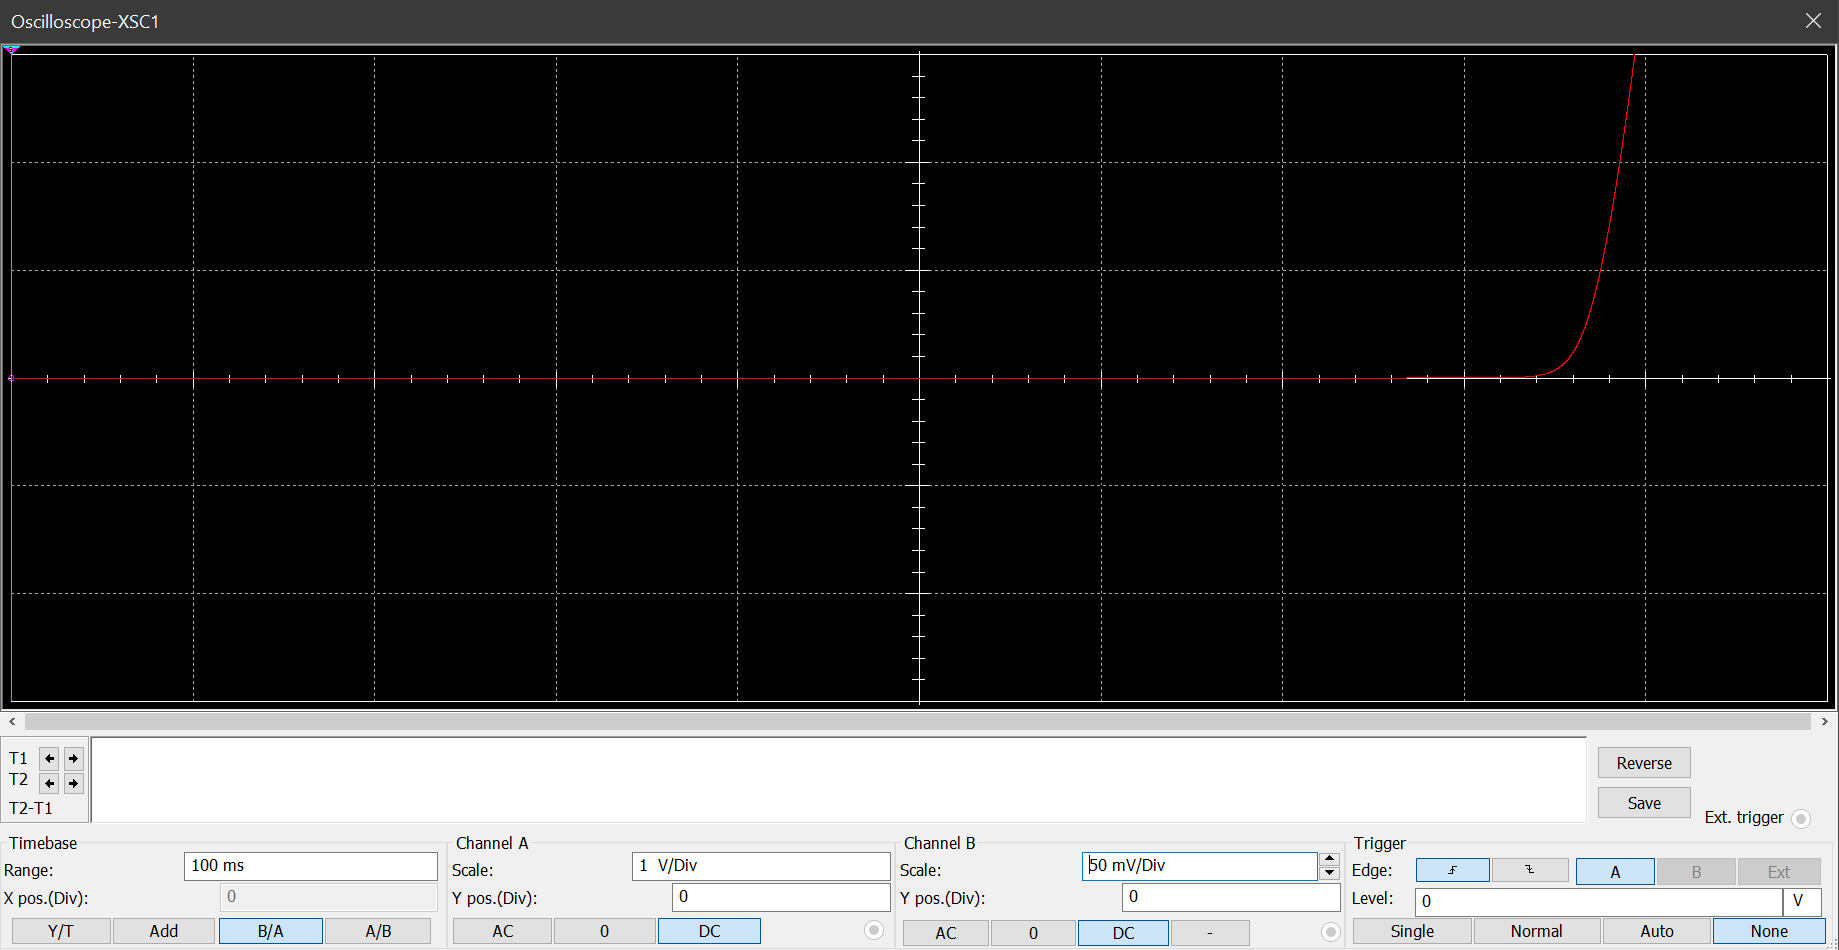
\includegraphics[width=0.45\textwidth]{blue_osc.png} }}%
        \caption{ВАХ с осциллограммы.}%
    \label{fig:example}
\end{figure}

Данные ВАХ совпадают с построенными поточечно графиками в предыдущим заданиях. \\
\ \\
В заключительном задании необходимо рассчитать величину ограничевающего ток через светодиод(возьмем исследованный выше $LED_{red}$) резистора $R_{load}$, с учетом заданных значений яркости и справочных данных $I_{d_{max}} = 0.03 \ A$, $V_{d_{max}} = 2.2 \ V$, $P_{d_{max}} = 0.066 \ W$. \\

\begin{figure}[H]
    \centering
    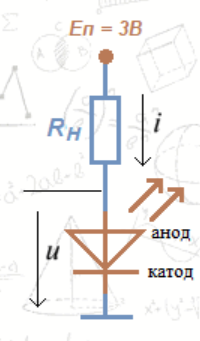
\includegraphics[width=0.2\textwidth]{last_scheme.png}
    \caption{Схема включения светодиода.}
    \label{fig:last_scheme}
\end{figure}

\begin{figure}[H]
    \centering
    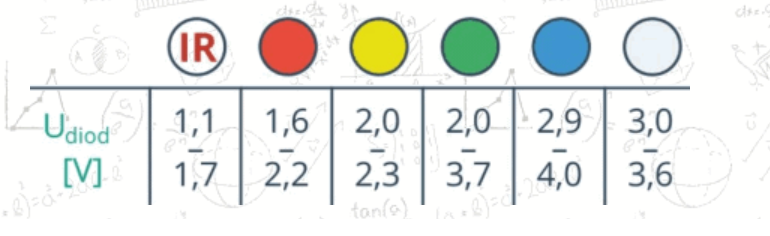
\includegraphics[width=0.45\textwidth]{colors_diod.png}
    \caption{Цветовая классификация.}
    \label{fig:colors_diod}
\end{figure}

Так как мы выбрали красный светодиод, то по цветовой классификации он имеет прямое падение напряжения в пределах $[1.6; \ 2.2] \ V$. \\
Необходимость ограничивающего резистора $R_{load}$(параметры которого необходимо рассчитать) обуславливается тем, что напрямую светодиод нельзя подключать к источнику питания, так как при значительных напряжениях светодиод может выйти из строя. Также необходимо, чтобы рассеиваемая мощность светодиодом не превышала $P_{d_{max}}$. \\
Итого, рабочая область светодиода будет ограничена так:

\begin{figure}[H]
    \centering
    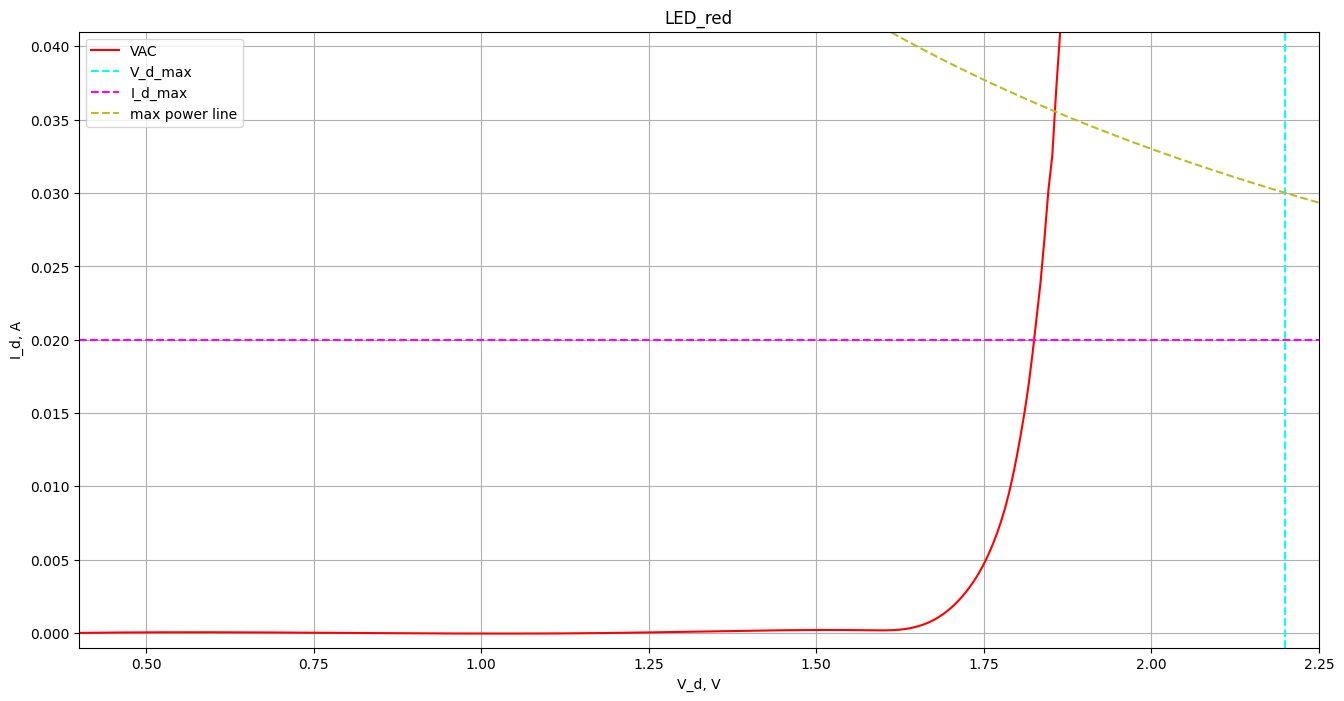
\includegraphics[width=\textwidth]{work_area_custom.png}
    \caption{Рабочая область светодиода.}
    \label{fig:work_area_custom}
\end{figure}

Рассчитаем рабочий ток $I_w$ и рабочее напряжение $V_w$ на светодиоде. \\
Пусть $E_{in} = 2.15 \ V$, тогда по 2 закону Кирхгофа:
\[
    E_{in} = I_w R_{load} + V_w \Rightarrow I_w = \frac{E_{in} - V_w}{R_{load}},
\]
построим данную прямую по двум точкам: первая - $(V_1 = 2.15 \ V, \ I_1 = 0 \ A)$, для второй точки зададимся током, не превышающим $I_{d_{max}}$, например $I_2 = 0.015 \ A$. Тогда для второй точки получаем:
\[
    V_2 = 0 \ V, \ I_2 = \frac{E_{in}}{R_{load}} = 0.015 \Rightarrow R_{load} = 143,3 \ Ohm.
\]
Проведем на графике данную \emph{нагрузочную прямую} по вычисленным 2-м точкам и отметим точку пересечения её с ВАХ - \emph{рабочая точка}. \\
\begin{figure}[H]
    \centering
    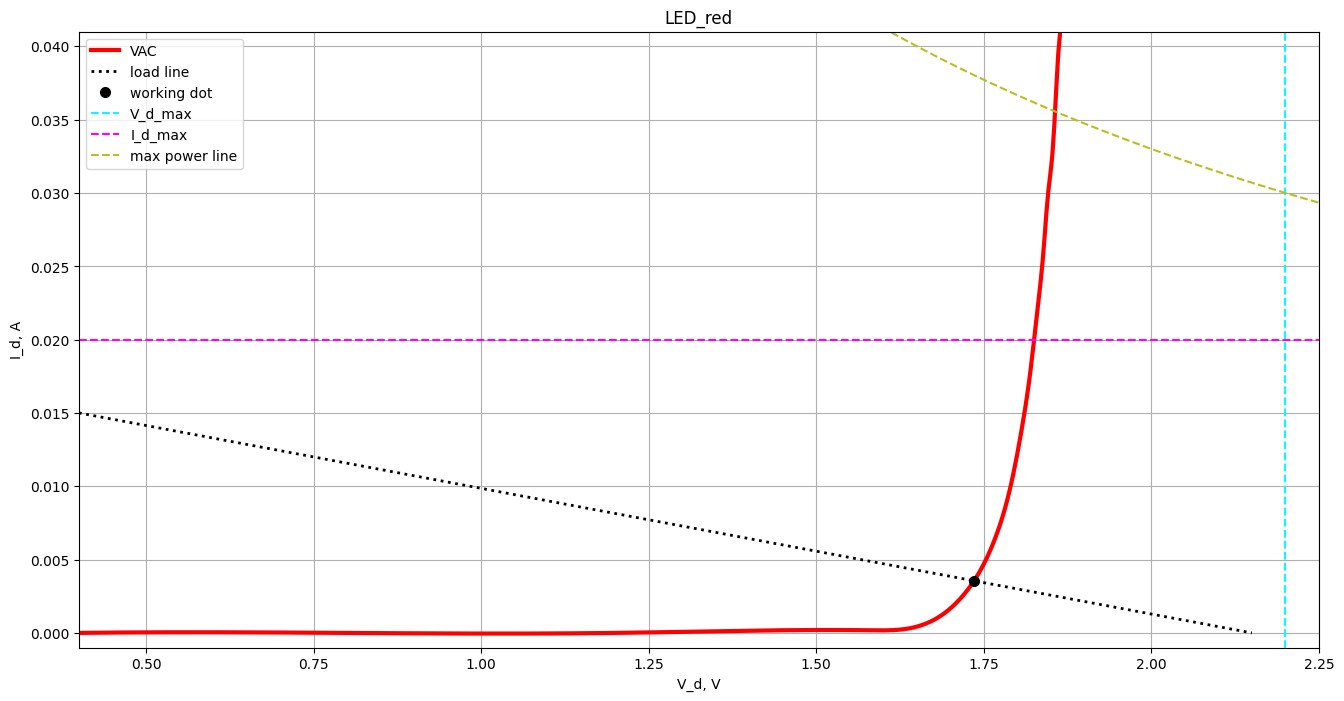
\includegraphics[width=\textwidth]{work_area_custom_w_ll_and_wd.png}
    \caption{Нагрузочная прямая с рабочей точкой.}
    \label{fig:work_area_custom_w_ll_and_wd}
\end{figure}
Координаты рабочей точки: $V_w = 1.73490982 \ V, \ I_w = 0.00351158 \ A$.\\
Теперь вычислим сопротивление:
\[
    R_{load} = \frac{E_{in} - V_w}{I_w} = 118.2 \ Ohm.
\]

\subsubsection*{Выводы}
В данной лабораторной работе исследовались диоды. Диод - двухэлектродный электронный компонент, обладающий различной электрической проводимостью в зависимости от полярности приложенного к диоду напряжения. Диоды обладают нелинейной несимметричной вольт-амперной характеристикой. \\
Соответственно в первых двух частях работы требовалось смоделировать прямой и обратный проход 4 видов диодов и построить их ВАХ. Данные ВАХ действительно нелинейны и несимметричны. Это происходит из-за того, что при приложении прямого напряжения (прямой проход) диод открыт (через диод течёт прямой ток, диод имеет малое сопротивление), а если к диоду приложено обратное напряжение (катод имеет положительный потенциал относительно анода), то диод закрыт (сопротивление диода велико, обратный ток мал, и может считаться равным нулю во многих практических случаях). \\
\ \\
В последней части работы проивзодился расчет каскада подключения светодиода (было найдено сопротивление ограничевающего резистора в цепи). Рабочая точка (определяющая режим работы прибора по постоянному току) была найдена как пересечение нагрузочной линии и ВАХ светодиода. Далее, исходя из 2 закона Кирхгофа было найдено значение сопротивления.

\end{document}